\documentclass[12pt,french]{article}

\usepackage[T1]{fontenc}
\usepackage[french]{babel}
\usepackage[utf8]{inputenc}
\usepackage{amsmath}
\usepackage{amssymb}
\usepackage{amsthm}
\usepackage{hyperref}
\usepackage{graphicx}

\title{Rapport Projet Informatique du Métro}
\author{
  Bouarah Romain \and
  Langdorph Matthieu \and
  Ketels Lucas \and
  Souffan Nathan
}


\begin{document}
\maketitle

Dans le cadre du Projet Informatique du 4ème semestre, voici le projet Métro. Ce programme permet de donner le trajet le plus court lors d'un déplacement sur un réseau de métro, représenté par un graphe. Ce programme a été codé en Java.  
\newpage
\tableofcontents

 
\newpage

\part{Guide d'utilisation du programme}
Voici des indications pour utiliser notre programme "metro". Nous l'avons conçu avec Maven, JUnit et Java.

\section{Installation}
Avant d'installer le programme, il faut vérifier bien avoir Java JDK, Maven et JUnit d'installer sur son ordinateur. Sinon les installer. Il faut également vérifier que les versions sont suffisament à jour, version au moins 8.0 pour Java, au moins 3.6 pour Maven, et au moins 4.11 pour JUnit.
Vous pouvez alors cloner le projet depuis master dans les fichiers de votre ordinateur.
Vous êtes alors prêt pour utiliser "metro".

\section{Utilisation}
Une fois la partie installation effectuée, vous pouvez compiler et exécuter "metro".
Se placer dans le répertoire adapté et se positionner sur master(par défaut).
Pour compiler le projet dans son intégralité, il faut utiliser la commande "make".
Il y a la possibilité de compiler juste datamodel ou le webserver, en faisant suivre leur nom après "make".
On peut compiler les tests avec "make test".
"make clean" supprime tous les fichiers produits pendant la compilation.

Pour exécuter le programme : on peut soit avoir une version minimale sur le terminal avec la commande "make run\_terminal". Sinon on peut avoir la version site Web en utilisant la commande "make run".

Nous allons donc voir comment utiliser le webserver "metro" dans la section suivante.

Nous avons également l'option d'afficher le graphe du réseau d'une ville en utilisant la commande "make export\_to\_dot ARGS="NomDeLaVille" ". Notons que les réseaux de métro des villes de Lille, Lyon, Marseille, Rennes, Toulouse, Paris, et des aéroports de Charles de gaulle et Orly.

\section{Exemple d'exécution}
Nous compilons donc avec la commande "make".
Nous lançons ensuite l'exécution avec "make run".

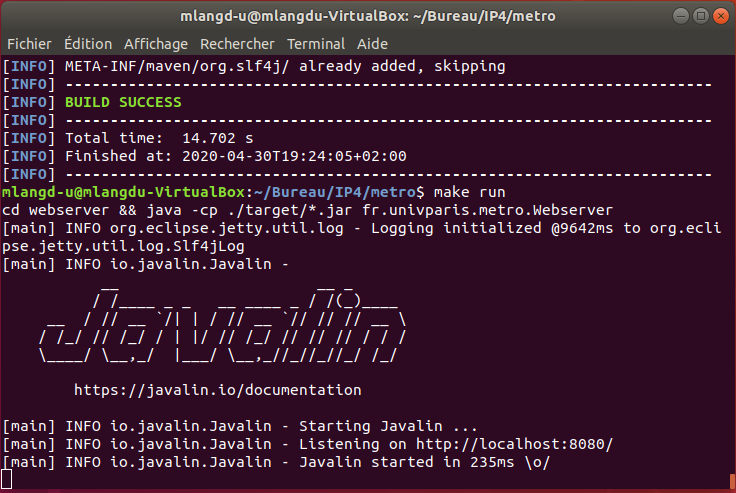
\includegraphics[height=5cm]{images/execute.png}

Il faut alors copier le lien(2ème ligne partant du bas) dans un navigateur web pour accéder au webserver de "metro". Cette page ci-dessous s'affiche et on sélectionne alors la ville de notre choix parmi celles possibles. On prend Paris dans cet exemple.

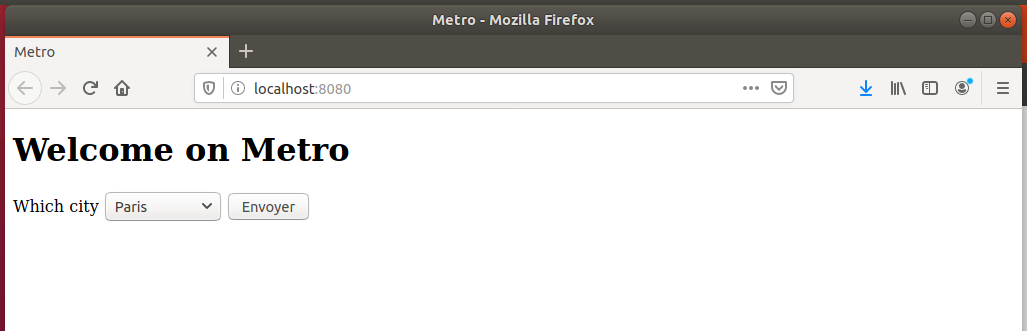
\includegraphics[height=3cm]{images/pageDAccueil.png}

Nous pouvons alors rechercher un itinéraire. Ici de Wagram à Ourcq. Trois options s'offrent à nous : utiliser Dijkstra(Shortest) pour trouver le plus court chemin, l'algorithme de Floyd ou l'algorithme de Bouarah pour trouver le plus court chemin avec un plafond de nombre de correspondances.

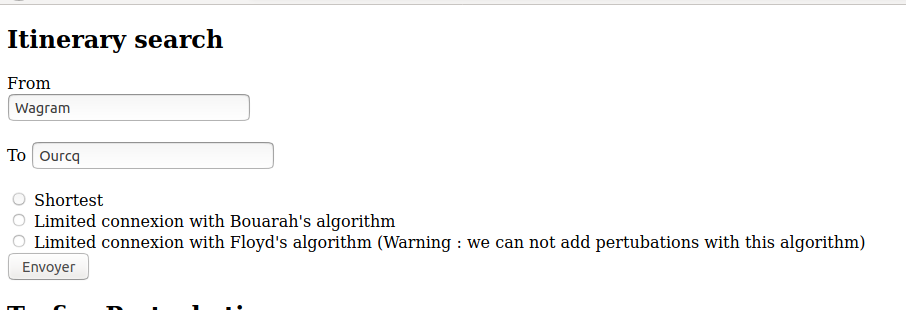
\includegraphics[height=3cm]{images/research.png}

Nous faisons ici une recherche avec Shortest. S'affichent alors plusieurs itinéraires dans l'ordre croissant en fonction des temps de trajets.

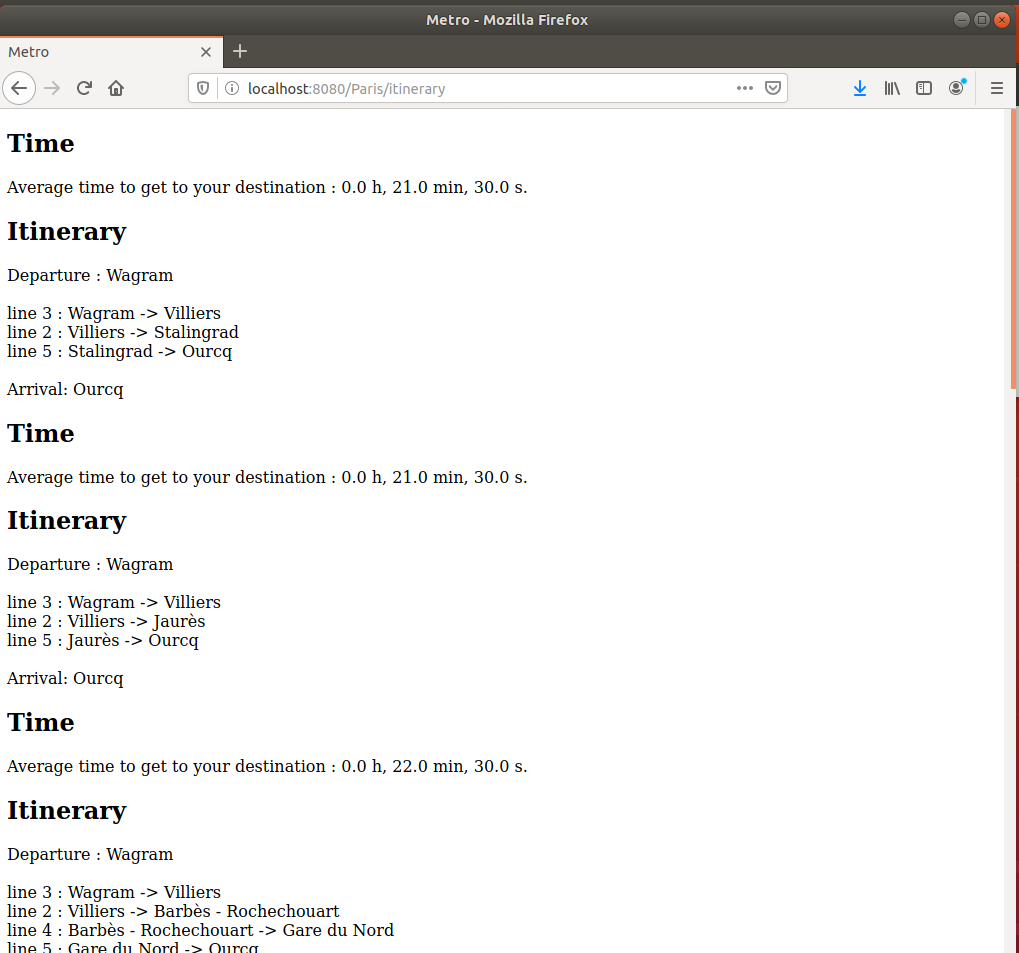
\includegraphics[height=8cm]{images/itineraryWithoutPbs.png}

Retournons à la page d'avant, on remarque la possibilité d'ajouter des perturbations de trafics. On peut arrêter ou ralentir une ligne ou une partie d'une ligne, fermer une station, fermer une ligne dans une station. Notre itinéraire précédent nous faisais passer par la ligne 2. Fermons donc la ligne 2 puis effectuons la même recherche de trajet entre Wagram et Ourcq.

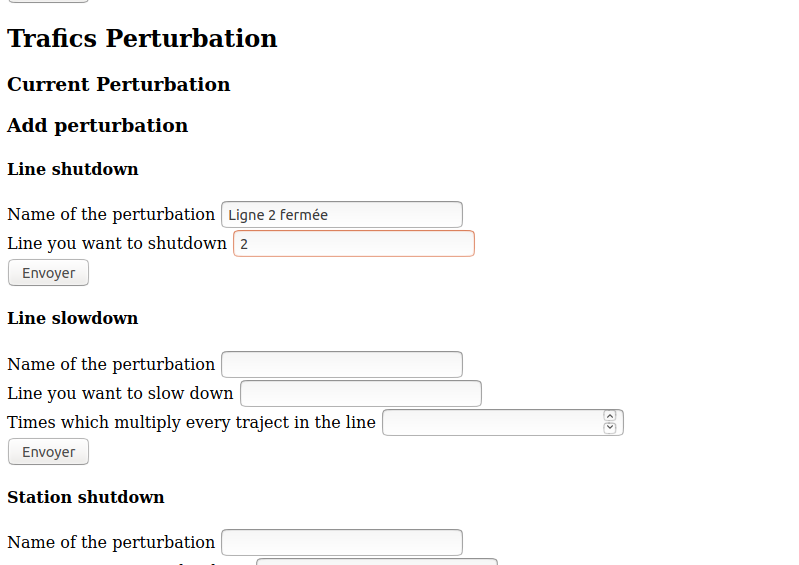
\includegraphics[height=4cm]{images/traficsPerturb.png}
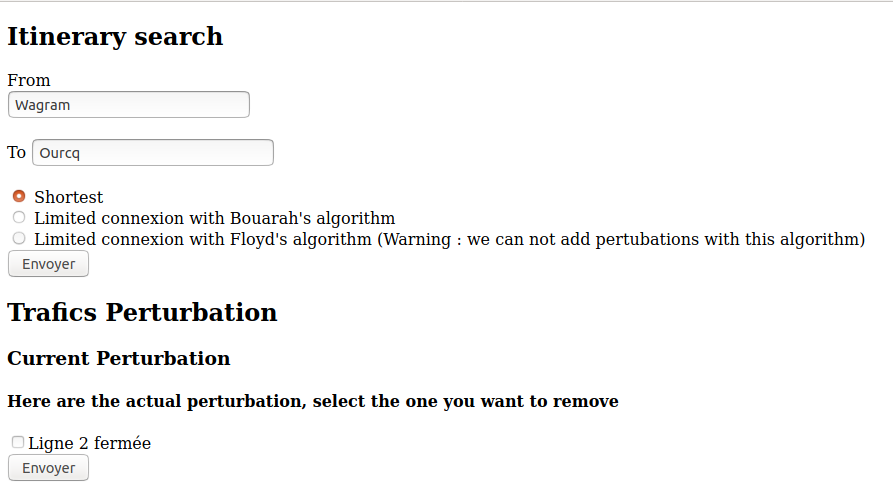
\includegraphics[height=4cm]{images/researchWithPbs.png}

On peut à présent voir le trajet le plus court sachant que la ligne 2 est fermée.

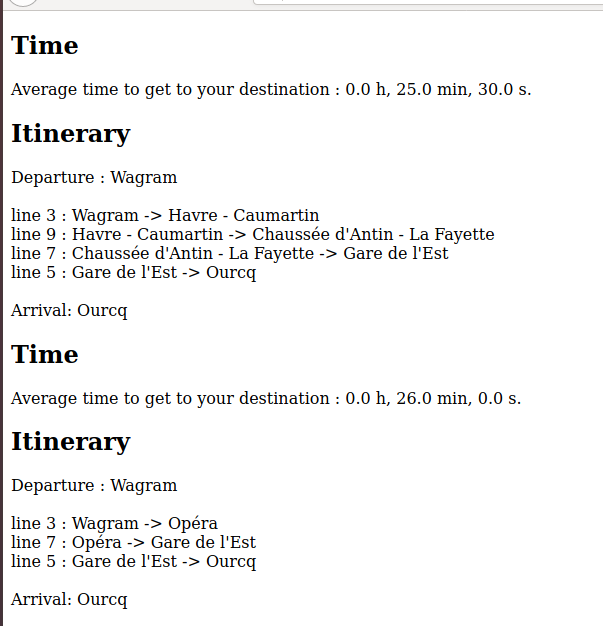
\includegraphics[height=8cm]{images/itineraryWithPbs.png}

Retournons maintenant à la page d'avant, allons en bas de page, et on peut voir qu'une section "Statistics" propose un lien vers une page affichant les statistiques du réseau de métro de la ville sélectionnée au préalable.

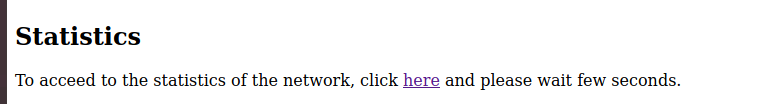
\includegraphics[height=2cm]{images/acceedStats.png}

Voici l'affichage de cette page :

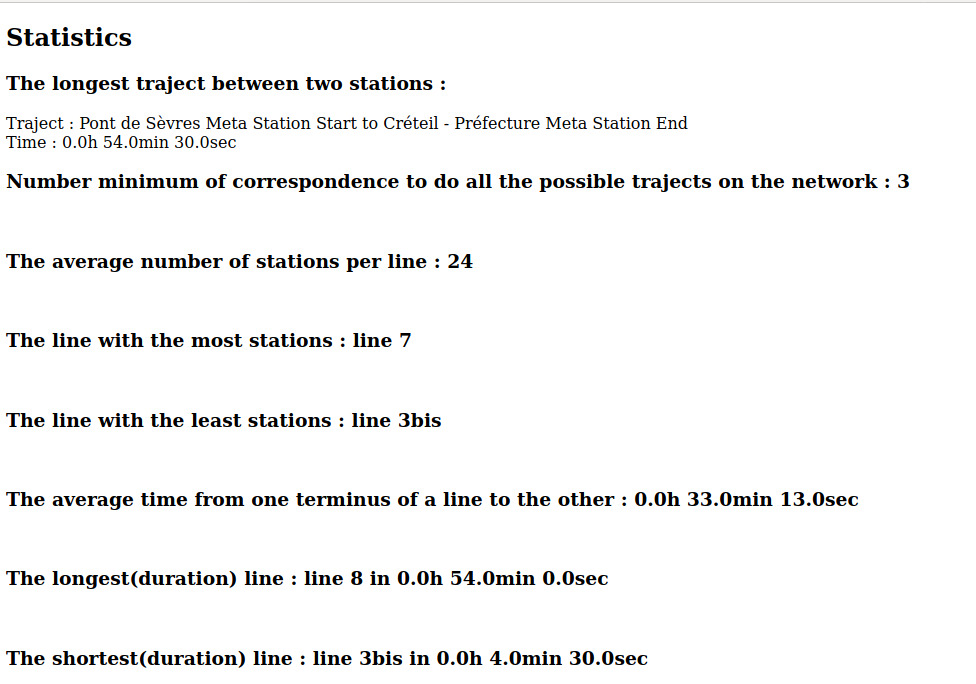
\includegraphics[height=6cm]{images/stats.png} 

Voici la fin de cet exemple d'utilisation de "metro" via son webserver.


 
\newpage

\part{Projet Métro}

\section{Présentation générale}
\subsection{Modélisation}
\subsection{Organisation}
\subsection{Problèmes rencontrés}


\section{Le projet dans ses grandes lignes}
\subsection{Les différents algorithmes}
\subsection{Structure des classes}
Diagramme des classes



\end{document}
